% ----------------------------------------------------------------------------------------------------------
% Packages
% ----------------------------------------------------------------------------------------------------------

\documentclass[12pt,a4paper,bibliography=totocnumbered,listof=totocnumbered]{scrartcl}
\usepackage[english]{babel}
\usepackage[utf8]{inputenc}
\usepackage{amsmath}
\usepackage{amsfonts}
\usepackage{amssymb}
\usepackage{graphicx}
\usepackage{fancyhdr}
\usepackage{tabularx}
\usepackage{geometry}
\usepackage{setspace}
\usepackage[right]{eurosym}
\usepackage[printonlyused]{acronym}
\usepackage{subfig}
\usepackage{floatflt}
\usepackage[usenames,dvipsnames]{color}
\usepackage{colortbl}
\usepackage{paralist}
\usepackage{array}
\usepackage{titlesec}
\usepackage{parskip}
\usepackage[right]{eurosym}
\usepackage[subfigure,titles]{tocloft}
\usepackage[pdfpagelabels=true]{hyperref}
\usepackage{mathdots}
\usepackage{listings}
\usepackage{lipsum}
\usepackage{booktabs}
\usepackage{fix-cm}
\usepackage{rotating}
\usepackage{pdflscape}
\usepackage[labelfont=bf]{caption}
\captionsetup{labelfont=bf}

% ----------------------------------------------------------------------------------------------------------
% Packages
% ----------------------------------------------------------------------------------------------------------


\lstset{basicstyle=\footnotesize, captionpos=t, breaklines=true, showstringspaces=false, tabsize=2, frame=lines, numbers=left, numberstyle=\tiny, xleftmargin=2em, framexleftmargin=2em}
\makeatletter
\def\l@lstlisting#1#2{\@dottedtocline{1}{0em}{1em}{\hspace{1,5em} Lst. #1}{#2}}
\makeatother



\geometry{a4paper, top=27mm, left=35mm, right=15mm, bottom=35mm, headsep=10mm, footskip=12mm}

% ----------------------------------------------------------------------------------------------------------
% Packages
% ----------------------------------------------------------------------------------------------------------


\hypersetup{unicode=false, pdftoolbar=true, pdfmenubar=true, pdffitwindow=false, pdfstartview={FitH},
	pdftitle={Master Thesis},
	pdfauthor={Felix Gutmann},
	pdfsubject={Bachelor Thesis},
	pdfcreator={\LaTeX\ with package \flqq hyperref\frqq},
	pdfproducer={pdfTeX \the\pdftexversion.\pdftexrevision},
	pdfkeywords={Bachelor Thesis},
	pdfnewwindow=true,
	colorlinks=true,linkcolor=black,citecolor=black,filecolor=magenta,urlcolor=black}
\pdfinfo{/CreationDate (D:20110620133321)}
\DeclareMathOperator*{\argmin}{arg\,min}
\begin{document}

\titlespacing\section{0pt}{12pt plus 4pt minus 2pt}{0pt plus 2pt minus 2pt}
\titlespacing\subsection{0pt}{30pt plus 4pt minus 2pt}{0pt plus 2pt minus 2pt}
\titlespacing\subsubsection{0pt}{12pt plus 4pt minus 2pt}{0pt plus 2pt minus 2pt}
% Headers and footers

\renewcommand{\sectionmark}[1]{\markright{#1}}
\renewcommand{\leftmark}{\rightmark}
\pagestyle{fancy}
\lhead{}
\chead{}
\rhead{\thesection\space\contentsname}
%\lfoot{Complex Economic Systems - An analytical approach to Input-Output tables\newline}
\cfoot{}
\rfoot{\ \linebreak \thepage}
\renewcommand{\headrulewidth}{0.4pt}
\renewcommand{\footrulewidth}{0.4pt}

% ----------------------------------------------------------------------------------------------------------
%Prefix
% ----------------------------------------------------------------------------------------------------------

\renewcommand{\thesection}{\Roman{section}}
\renewcommand{\theHsection}{\Roman{section}}
\pagenumbering{Roman}

% ----------------------------------------------------------------------------------------------------------
% Title
% ----------------------------------------------------------------------------------------------------------

\thispagestyle{empty}
\begin{center}
	
\includegraphics[width=\textwidth]{Pictures/logo01.jpg}\\
	\vspace*{2cm}
	\vspace*{2cm}
	\Huge
	\textbf{Master Thesis}\\
	\vspace*{0.5cm}
	\large
	\textbf{Topic:}\\
	\vspace*{1cm}
	\textbf{Unsupervised learning in decision making}\\
	\vspace*{2cm}
\end{center}	

$\vspace{6cm}$
\begin{tabbing}
\hspace*{1cm}\=\hspace*{3.2cm}\=\hspace*{3cm}\=\hspace*{2.7cm}\= \kill
\onehalfspacing
\textbf{Author:} \>\> Domagoj Fizulic\\
\textbf{} \>\> Felix Gutmann\\
\textbf{Student number:} 	\>\> 125604\\
\textbf{} 	\>\> 125584\\
\textbf{Program:} \>\> M.S. Data Science\\
\textbf{E-Mail:} \>\> domagoj.fizulic@barcelonagse.eu\\
\textbf{} \>\> felix.gutmann@barcelonagse.eu
\end{tabbing}
\vspace{1cm}


\pagebreak
% ----------------------------------------------------------------------------------------------------------
% Abstract
% ----------------------------------------------------------------------------------------------------------


\onehalfspacing




\pagebreak

% ----------------------------------------------------------------------------------------------------------
% Index
% ----------------------------------------------------------------------------------------------------------


\renewcommand{\cfttabpresnum}{Tab. }
\renewcommand{\cftfigpresnum}{Fig. }
\settowidth{\cfttabnumwidth}{Fig. 10\quad}
\settowidth{\cftfignumwidth}{Fig. 10\quad}

\titlespacing{\section}{0pt}{12pt plus 4pt minus 2pt}{2pt plus 2pt minus 2pt}
\singlespacing
\rhead{Table of contents}
\renewcommand{\contentsname}{I Table of Contents}
\phantomsection
\addcontentsline{toc}{section}{\texorpdfstring{I \hspace{0.35em}Table of Contents}{Table of Contents}}
\addtocounter{section}{1}


% ----------------------------------------------------------------------------------------------------------
% Table of contents
% ----------------------------------------------------------------------------------------------------------

\setcounter{page}{1}

\rhead{Table of Contents}

	\tableofcontents


\pagebreak
% ----------------------------------------------------------------------------------------------------------
% List of figures
% ----------------------------------------------------------------------------------------------------------

\rhead{List of Figures}

	\listoffigures
	
	
\pagebreak
% ----------------------------------------------------------------------------------------------------------
% List of tables
% ----------------------------------------------------------------------------------------------------------

\rhead{List of Tables}

	\listoftables
	

\pagebreak
%----------------------------------------------------------------------------------------------------------
% List of Listings
% ----------------------------------------------------------------------------------------------------------

\rhead{List of Listings}
\renewcommand{\lstlistlistingname}{List of Listings}
{\labelsep2cm\lstlistoflistings}
\pagebreak

%----------------------------------------------------------------------------------------------------------
% List of Symbols
% ---------------------------------------------------------------------------------------------------------

\renewcommand{\arraystretch}{1.5}	
\section{List of mathematical symbols}
\rhead{List of mathematical Symbols}

\begin{tabular}{p{6cm}p{9cm}}
\textbf{Symbol} 		& 		\textbf{Meaning} \\
\midrule
\vspace{0.3cm} & \vspace{0.3cm} 			\\
$a_t$				  & Action at time t			\\
$Q(a)_t$	& Value function at time t \\
$\epsilon$			& Probability of exploration in epsilon greedy \\
$\alpha$ & Learning rate \\ 
$\tau$ & Softmax parameter \\
$H(X) $ &  Entropy of a  discrete random variable $X$ \\ 
$ \mathbb{R}_0^+$ & Positve real numbers including zero 
\end{tabular}

\pagebreak

%----------------------------------------------------------------------------------------------------------
% List of abbreviations
% ---------------------------------------------------------------------------------------------------------

\section{List of abbreviations}
\rhead{List of Abbreviations}

\begin{tabular}{p{6cm}p{9cm}}
\textbf{Abbreviations} & \textbf{Description} 										\\
\midrule
\vspace{0.3cm} & \vspace{0.3cm} 														\\ 
\end{tabular}

\newpage

% ----------------------------------------------------------------------------------------------------------
% Prefix 2
% ----------------------------------------------------------------------------------------------------------

% Title spacing

\titlespacing{\section}{0pt}{12pt plus 4pt minus 2pt}{-6pt plus 2pt minus 2pt}
\titlespacing{\subsection}{0pt}{12pt plus 4pt minus 2pt}{-6pt plus 2pt minus 2pt}
\titlespacing{\subsubsection}{0pt}{12pt plus 4pt minus 2pt}{-6pt plus 2pt minus 2pt}

% Header

\renewcommand{\sectionmark}[1]{\markright{#1}}
\renewcommand{\subsectionmark}[1]{}
\renewcommand{\subsubsectionmark}[1]{}
\lhead{Chapter \thesection}
\rhead{\rightmark}

\onehalfspacing

\renewcommand{\thesection}{\arabic{section}}
\renewcommand{\theHsection}{\arabic{section}}
\setcounter{section}{0}
\pagenumbering{arabic}
\setcounter{page}{1}

%RGB Colour set

\definecolor{persblue}{rgb}{0.0862745,0.211765,0.360784}
\definecolor{persred}{rgb}{0.388235,0.145098,0.137255}
\definecolor{persgray}{rgb}{0.501961,0.501961,0.501961}
\definecolor{persgreen}{rgb}{0.054902,0.411765,0.352941}

%---------------------------------------------------------------------------------------------------------
% 1. Introduction
%---------------------------------------------------------------------------------------------------------

\section{Introduction and conceptual approach}

Learning is a complex procedure. The learning procedure can affected due to social conditions... 


\pagebreak
%---------------------------------------------------------------------------------------------------------
% 2. Literature
%---------------------------------------------------------------------------------------------------------

\section{Relevant Literature}


\pagebreak
%---------------------------------------------------------------------------------------------------------
% 3. Simmulation
%---------------------------------------------------------------------------------------------------------

\section{Theoretical Backround and experiments}

In this section we provide ... 

\subsection{Simmulation experiment design}

Before analysing real data we run some simmulation experiments to indentify adequat approaches to model our data. To generate data artificially we follow a reinforcement learning and multi arm bandit approach where we let an agent learn the distribution of a simulated data set. The procedure is illustrated in figure \ref{fig:flow}. To keep things simple we draw a set of rewards from a normal distribution. We let several agents with different parameter setting process the reward data. From this procedure we obtain for each agent a time series of choices. 

 \begin{figure}[!htb]
	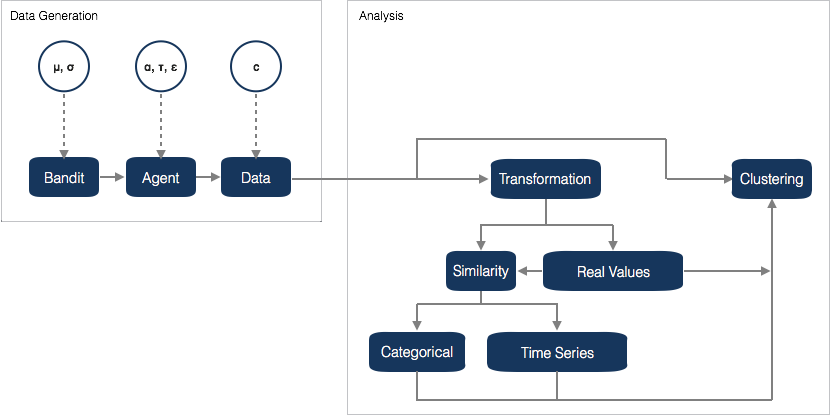
\includegraphics[width=\textwidth]{Pictures/flow01.png}
	\caption{Flowchart experiment desgin}
	\label{fig:flow}
\end{figure}

Concerning our data we find two main challanges. First, our data have a categorical nature. Furhtermore, the learning process also imposes a time series dependence on the data. We address this issue in the following ways. 
The first approach is to map the series of choices to a real valued series. For each time step we can compute \textit{Shannon's Entropy} based on the empirical probability of the choices. Let $X$ be a discrete random variable with probability $p$, then the entropy is defined as:
\begin{flalign}
H(X) := -\sum_{i=1}^{N} p_i \log_2 p_i
\end{flalign}
Entropy gives measure on how random a random variable behaves. Therefore, transforming choices to sequentiel entropy is to discriminate individuals by the randomness

\subsection{Reinforcement Learning backround and multi arm bandits}

\textit{Reinforcement Learning} (RIL) is a branch of \textit{Machine Learning} try model how an artificial agents interact with its environment and learns from the process over time. \\
In particular an agents is confronted with the task of choosing sequently from a set of choices. In comparison to \textit{supervised learning}, where an agent is learning based on set of examples an agent in RIL doesn't have any knowledge about the system apriori. Therefore, it has to learn the nature of the system by sequentially interacting with its environment and keeping tack of the obtained information. Since the agent doesn't have any apriori information about the system it has to explore new possible action and so has to deviate from the optimal action. Furthermore, it has to keep track of value of each action he did so far. So the main task of the agent is to balance exploration and explotation. 
There are to basic approaches to model this trade-off; An \textit{"Epsilon-Greedy"} selection method and Soft \textit{"Softmax"} selection method. Before explaining both cocepts we introduce the value function for a given action $a$. Therefore,  let $Q_t(a)$ be the value function of action defined as:
\begin{flalign}
Q_t(a) := \frac{R_1 + R_2 + \dots + R_{K_\alpha}}{K_\alpha}
\end{flalign}
The value function is the average over rewards. 

Considering now epsilon greedy action selection mehtod: The rule in general is to select the next action as the current current highest value function. However, to model exploration we introduce a random element to deviate from that greedy strategy. Following that the next action
\begin{flalign}
a_{t+1} = \begin{cases} 
\text{random action} & \text{, with probability } \epsilon \\
\arg \max_i Q_t(i) & \text{, with probability } 1-\epsilon
\end{cases}
\end{flalign}
where $\epsilon \in [0,1]$ is a parameter controling the random behaviour of the agent. 

In the softmax action selection method compute for each action a probability (also called \textit{Boltzmann Distribution)}. The probability for action a is computed by:
\begin{flalign}
P(a_{t}|X) = \frac{e^{\frac{Q_t(a)}{\tau}}}{\sum_{i}^{K} e^{\frac{Q_t(i)}{\tau}}}
\end{flalign}
In each iteration the next action of the agent is drawn with probability $p_a$: 
\begin{flalign}
a_{t+1} \sim p_a
\end{flalign}

After selecting an action the agent is updating its believe of the chosen action. Formally the update rule is defined
\begin{flalign}
Q(a)_{k+1} = Q(a)_k + \alpha \left[ R(a)_k -  Q(a)_k	 \right],
\end{flalign}
where $\alpha$ is a is the  non negativ \textit{learning rate} defining how much the current action is affecting the believes.

\subsection{Unsupervised Learning}

We consider several unsupervised clustering techniques. A technical description for all of the is provided in 

\begin{table}[!htb]
	\centering
	\begin{tabular}{|c| c| c |}
		\toprule \toprule
		\textbf{Algorithm} & Input & Datatype  \\
		\hline
		Spectral Clustering & Similarity Matrix & -  \\
		Affinity Propagation & Similarity Matrix & -  \\
		K-Means Clustering & Data Matrix & -  \\
		Ward Clustering & Data Matrix & -  \\
		PCA + 	Ward Clustering   & Data Matrix & -  \\
		\bottomrule
	\end{tabular}
	\caption{Overview clustering algorithms}
\end{table}
	
\subsection{Simmulation results}


%---------------------------------------------------------------------------------------------------------
% 4. Data
%---------------------------------------------------------------------------------------------------------

\section{Data Analysis}

\subsection{Data Description}

\subsection{Results}

%---------------------------------------------------------------------------------------------------------
% 5. Data
%---------------------------------------------------------------------------------------------------------

\section{Conclusion}

\pagebreak
% ----------------------------------------------------------------------------------------------------------
% Literature
% ----------------------------------------------------------------------------------------------------------

\renewcommand\refname{List of Literature}

\bibliographystyle{apalike}

\bibliography{bib}


\pagebreak

%----------------------------------------------------------------------------------------------------------
% Appendix
% ---------------------------------------------------------------------------------------------------------
\lhead{Appendix \thesection}
\rhead{}
\pagenumbering{Alph}
\setcounter{page}{1}

\begin{appendix}
	
\section*{Appendix}
\phantomsection
\addcontentsline{toc}{section}{Appendix}
\addtocontents{toc}{\vspace{-0.5em}}

\subsection*{Metrics and Similarities}

This part of the appendix formally defines metrics and similarities and dissimilarities (proximity) used in this paper. We first define some basic general concepts followed by a description of the applied distance and similarity concepts. 

Let $\boldsymbol{X}$ be a dataset and let $\boldsymbol{x_i},\boldsymbol{x_j}$ be two datapoints, such that $\boldsymbol{x_i},\boldsymbol{x_j} \in \boldsymbol{X}$. 

A distance function assign for pairs a points a non negative real number as distance. $d:\boldsymbol{X}\times \boldsymbol{X} \mapsto \mathbb{R}_0^+$. Formally if the following properties are additionally staisfied the distance is also metric.

\begin{enumerate}
	\setlength{\itemsep}{-5pt}
	\item $d(\boldsymbol{x_i},\boldsymbol{x_j}) \ge 0$
	\item $d(\boldsymbol{x_i},\boldsymbol{x_i}) \ge 0$
	\item $d(\boldsymbol{x_i},\boldsymbol{x_j}) = d(\boldsymbol{x_j},\boldsymbol{x_i}) $
	\item $d(\boldsymbol{x_i},\boldsymbol{x_j}) \le d(\boldsymbol{x_i},\boldsymbol{x_j})+ d(\boldsymbol{x_j},\boldsymbol{x_i}) $
\end{enumerate}

A distance can be seen as a measure for disimilarity of two points. Besides distance some algorithms operate on a \textit{similarity} matrix. Formally a similarity is a function  $ S : \boldsymbol{X} \times \boldsymbol{X} \mapsto [0,1] $. Also for similarity we can define the following properties:

\begin{enumerate}
	\setlength{\itemsep}{-5pt}
	\item $0 \le S(\boldsymbol{x_i},\boldsymbol{x_j}) \le 1, \text{for } i \neq j$
	\item $S(\boldsymbol{x_i},\boldsymbol{x_j}) = 1$
	\item $S(\boldsymbol{x_i},\boldsymbol{x_j}) = S(\boldsymbol{x_j},\boldsymbol{x_i})$
\end{enumerate}

Once we have computed distance or a similarity we can compute for two data points we can use this information to transform it to a similarity or the distance vice versa:

\begin{flalign}
S(\boldsymbol{x_i},\boldsymbol{x_j}) = \frac{1}{1+d(\boldsymbol{x_i},\boldsymbol{x_j}) } \hspace{0.5cm} \Leftrightarrow \hspace{0.5cm} d(\boldsymbol{x_i},\boldsymbol{x_j}) =  \frac{1}{S(\boldsymbol{x_i},\boldsymbol{x_j})} -1 
\end{flalign}


\pagebreak

\subsection*{Principal Components and Multidimensional Scaling}


\pagebreak
\subsection*{Spectral Clustering}

For the spectral clustering algorithm we formally introduce some graph notation. If not stated otherwise the following derivation follows [SOURCE]. In the following we consider a weighted and simple undirected graph. 
\begin{flalign}
G &= \{V,E\} \\
V & = \{ v_1,\dots,v_n \} \\
E & = \{e_1,\dots,e_n\} 
\intertext{Furthermore let the graph has a weighted and symetric ($|V| \times |V|$) adjacency matrix, such that:}
\boldsymbol{W} &= \begin{cases} 
w_{i,j} & \text{,if } v_iv_j \in E \\
0 & \text{otherwise }
\end{cases}
\intertext{The \textit{degree} of a node is defined as the sum of edge weights of connected nodes. Formmally we denote the degree of node $i$ as:}
d_i &:= \sum_{j=1}^{n} w_{ij} = \sum_{i=1}^{n} w_{ij}
\intertext{Using the last expression we define matrix $\boldsymbol{D}$ as the diagonal matrix of the degress}
\boldsymbol{D} &:= diag(\boldsymbol{d})
\intertext{The algorithm works on the \textit{Laplacian} matrix defined by:}
\boldsymbol{L} &:= \boldsymbol{D} - \boldsymbol{W} 
\intertext{Former versions of the algorithm are applied on the graph laplcian. However, there were proposed newer versions using the so called \textit{normalized laplacian}. Since also the python version is using this package we will focus on this version of the algorithhm. Following that the normalized graph laplacian is defined as:}
\boldsymbol{L}_{norm} &:= \boldsymbol{D}^{1/2} \boldsymbol{L} \boldsymbol{D}^{1/2}  = \boldsymbol{I} - \boldsymbol{D}^{1/2} \boldsymbol{W} \boldsymbol{D}^{1/2}
\end{flalign}



\end{appendix}

\pagebreak
%----------------------------------------------------------------------------------------------------------
% End Document
%----------------------------------------------------------------------------------------------------------


\begin{sidewaystable}[!h]
	\centering
	\begin{tabular}{| l || c | c | c | c | c | c | c | c | c | c || c  |  c | c | c | c | c | }
		\toprule \toprule
		\textbf{Specification} &$\boldsymbol{\mu}$ & $\boldsymbol{\sigma}$ & \textbf{CL Size} & \textbf{SD} & \textbf{Decision} & $\boldsymbol{\alpha}$  &  $\boldsymbol{\tau}$  & \textbf{N} & \textbf{ALG} & \textbf{TRNS} &  \textbf{MI} & \textbf{NMI} &  \textbf{AMI} &  \textbf{CS} &  \textbf{HS } & \textbf{VMS}     \\
		\hline
		1 & -  & -& -& -& -& -& -& -& -& -& -& -& - & - \\
		\bottomrule
	\end{tabular}
	\caption{Overview Outcome }
\end{sidewaystable}


\end{document}